\documentclass[12pt]{article}
\usepackage{xcolor}
\usepackage{float}
\usepackage{listings}
\definecolor{vgreen}{RGB}{93, 145, 85}
\definecolor{vblue}{RGB}{31, 80, 179}
\definecolor{vorange}{RGB}{206, 114, 60}
\definecolor{backgroundColour}{rgb}{0.95,0.95,0.92}
\usepackage{graphicx}
\usepackage{indentfirst}
\usepackage[a4paper, total={6in, 8in}]{geometry}
\usepackage[colorlinks,linkcolor=blue,citecolor=blue]{hyperref}
\usepackage{fancyhdr}
\usepackage{xepersian}
\settextfont[BoldFont=BNazanin Bold.ttf]{BNazanin.ttf}
\setlatintextfont[BoldFont=timesbd.ttf]{times.ttf}
\renewcommand{\labelitemi}{$\bullet$}
\renewcommand{\labelitemii}{$\bullet$}
\lstdefinestyle{python-style}
{
	language=Python,
	basicstyle=\small\ttfamily,
	backgroundcolor=\color{backgroundColour},   
	keywordstyle=\color{vblue},
	identifierstyle=\color{black},
	commentstyle=\color{vgreen},
	stringstyle=\color{vorange},
	numbers=left,
	numberstyle=\tiny\color{black},
	numbersep=10pt,
	tabsize=8,
	showspaces=false,
	showstringspaces=false,
	showtabs=false,
	tabsize=4,
	breaklines=true,
	breakatwhitespace=true,
	literate=*{:}{:}1
}

\begin{document}

%title page%
\begin{titlepage}
	\begin{center}
		\textbf{ \Huge{به نام خدا}}
	
		\vspace{0.2cm}
	
		
\includegraphics[width=0.4\textwidth]{sharif.png}\\
		\vspace{0.2cm}
		\textbf{ \Huge{پروژه‌ی سوم}}\\
		\vspace{0.25cm}
		\textbf{ \Large{سیستم‌های عامل - دکتر اسدی و دکتر جلیلی}}
		\vspace{0.2cm}
		
		
		\large \textbf{دانشکده مهندسی کامپیوتر}\\\vspace{0.1cm}
		\large   دانشگاه صنعتی شریف\\\vspace{0.2cm}
		\large   ﻧﯿﻢ‌سال اول ۰۳-۰۴ \\\vspace{0.10cm}
		\large{گروه ۲۲ :}\\
		\large{آریان افضل‌زاده - \lr{401105572}}\\
		\large{میترا قلی‌پور - \lr{401106363}}\\
		\large{الینا هژبری - \lr{401170661}}\\
		\large{ملیکا علی‌زاده - \lr{401106255}}\\
	\end{center}
\end{titlepage}
%title page%

\newpage

%pages header
\pagestyle{fancy}
\fancyhf{}
\fancyfoot{}
\setlength{\headheight}{59pt}
\cfoot{\thepage}
\lhead{پروژه‌ی سوم}
\rhead{\hspace{0.87cm}
\includegraphics[width=0.1\textwidth]{sharif.png}\\
		دانشکده مهندسی کامپیوتر
}
\chead{سیستم‌های عامل}
%pages header

\newpage

\begingroup
\hspace{0.1cm}\Large\textbf{مقایسه‌ی تاثیر غیر همزمان‌سازی فراخوان‌های سیستمی و حذف سربار فراخوانی سیستمی در عملکرد ذخیره‌سازی}
\endgroup

\section*{مقدمه}
با پدید آمدن حافظه‌های سریع‌تر، سربار زمانی فراخوان‌های سیستمی برای درخواست‌های ورودی/خروجی حائز اهمیت شده است. پلتفرم \lr{SPDK} توسعه یافته است که با حذف برخی از سربارها در فراخوانی‌های سیستمی در لینوکس، سرعت دسترسی به دیسک‌های \lr{NVMe} را افزایش دهد. همچنین، \lr{RocksDB} پایگاه داده‌ی پرسرعت \lr{key-value}  برای محیط‌های ذخیره‌سازی سریع و پردازنده‌های چندهسته‌ای فراهم می‌کند.

\section*{اهداف}
\begin{enumerate}
	\item 
	آشنایی با پشته ذخیره سازی در سیستم‌عامل لینوکس
	\item
	شبیه‌سازی دیسک پرسرعت با پروتکل ارتباطی \lr{NVMe}
	\item 
	اجرای آزمون‌های عملکردی با \lr{RocksDB} و ابزار \lr{FIO}
	\item 
	آشنایی و استفاده از پلتفرم \lr{SPDK}
\end{enumerate}

\section*{صورت پروژه}
در این پروژه قصد داریم با استفاده از دیسک شبیه‌سازی شده \lr{NVMe} در شبیه‌ساز \lr{NVMeVirt}، تاثیر فراخوان‌های سیستمی \lr{io\_uring} و \lr{libaio} با \lr{SPDK} را بر اساس معیارهای \lr{IOPS}، \lr{Latency} و \lr{TailLatency} مقایسه کنیم. همچنین، برنامه‌ای محک  روی \lr{RocksDB} با استفاده از \lr{SPDK} اجرا و نتایج عملکرد را تحلیل خواهیم کرد.

\section*{گام‌های پروژه}
\begin{enumerate}
	\item 
	بررسی شبیه‌ساز \lr{NVMeVirt} و تهیه‌ی مستند از ساختار و مراحل نصب آن به همراه تفاوت روش‌های مختلف
	\item
ایجاد دیسک \lr{NVMeVirt\_NVM} و مشاهده‌ی عملکرد آن
	\item 
	اجرای ابزار \lr{FIO} روی دیسک شبیه‌سازی شده با مؤلفه‌های زیر
	\begin{figure}[H]
		\centering
		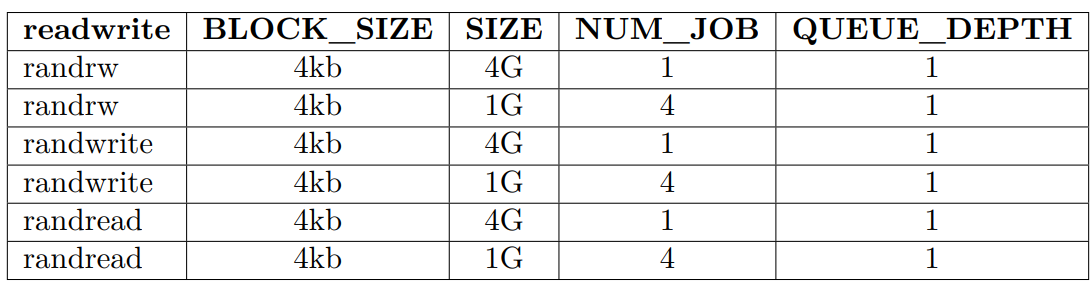
\includegraphics[scale=0.65]{./table}
	\end{figure}
	\item 
	نصب پلتفرم \lr{SPDK} و استفاده از پلاگین \lr{FIO} برای آزمایش
	\item 
	اجرای برنامه‌ای محک مانند \lr{db\_bench} روی \lr{RocksDB} با استفاده از \lr{SPDK}
	\item
	تحلیل و مقایسه‌ی نتایج و تهیه‌ی نمودار نمودار
\end{enumerate}

\newpage

\section*{گام اول پروژه}
\subsection*{\lr{NVMeVrit}}
\lr{NVMeVrit} برای شبیه‌سازی دستگاه‌های \lr{NVMe} در سطح \lr{PCIe} طراحی شده است تا از دید سیستم‌عامل میزبان، مانند یک دستگاه فیزیکی واقعی عمل کند. در معماری \lr{PCIe}، ریشه مجتمع \lr{PCIe Root Complex} ارتباط بین پردازنده و دستگاه‌های متصل به \lr{PCIe} را مدیریت می‌کند و اطلاعات پیکربندی آن‌ها را از طریق هدر پیکربندی \lr{PCIe} شناسایی می‌کند. \newline
\lr{NVMeVrit} برای معرفی یک دستگاه \lr{NVMe} مجازی، یک باس \lr{PCIe} مجازی ایجاد کرده و یک هدر پیکربندی \lr{PCIe} جعلی در حافظه رزرو‌شده ثبت می‌کند. این هدر، اطلاعات مورد نیاز برای شناسایی دستگاه، مانند \lr{Device ID} و \lr{Vendor ID} را ارائه می‌دهد. هنگام اسکن باس \lr{PCIe}، سیستم‌عامل میزبان این دستگاه را مانند یک \lr{NVMe} واقعی شناسایی کرده و درایور \lr{NVMe} را برای آن بارگذاری می‌کند، بدون اینکه نیازی به تغییرات سخت‌افزاری باشد. \newline
در دستگاه‌های واقعی، عملیات \lr{NVMe} از طریق تراکنش‌های \lr{PCIe} به سخت‌افزار \lr{NVMe} ارسال می‌شود. اما در \lr{NVMeVrit}، کنترلر \lr{NVMe} در حافظه رزرو‌شده سیستم شبیه‌سازی شده است. برای نظارت بر درخواست‌های \lr{I/O}، \lr{NVMeVrit} از یک رشته کرنل به نام \lr{Dispatcher} استفاده می‌کند که تغییرات در بلاک کنترل \lr{NVMe} را بررسی کرده و درخواست‌های \lr{I/O} را پردازش می‌کند. به جای استفاده از روش‌های مبتنی بر رویداد \lr{(event-driven)} که باعث ایجاد تأخیر می‌شوند، از پویش مداوم \lr{(busy-waiting)} برای کاهش تأخیر پردازش استفاده شده است. \newline
\begin{figure}[h]
    \centering
    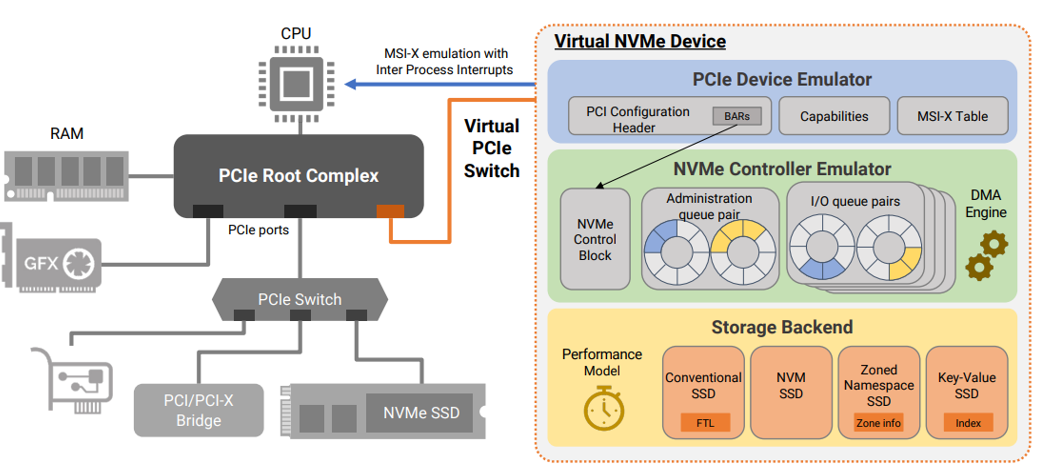
\includegraphics[width=0.8\textwidth]{NVMeVirt.png}
    \caption{شکل 1- معماری کلی \lr{NVMeVrit}. \lr{NVMeVrit} یک دستگاه \lr{NVMe} مجازی را از طریق گذرگاه و سوئیچ \lr{PCIe} مجازی می کند.}
\end{figure}
\newpage
\subsection*{بخش‌های کلیدی معماری \lr{NVMeVrit}}
\begin{enumerate}
    \item \textbf{شبیه‌سازی دستگاه \lr{PCIe}}: شامل ایجاد و مدیریت هدر پیکربندی برای دستگاه‌های مجازی.
    \item \textbf{کنترل بلاک \lr{NVMe}}: اطلاعات کنترلی در حافظه رزرو شده نگهداری می‌شود.
    \item \textbf{\lr{Dispatcher}}: درخواست‌های \lr{I/O} را بررسی کرده و به صف مناسب منتقل می‌کند.
    \item \textbf{\lr{I/O Workers}}: پردازش درخواست‌های \lr{I/O} بر اساس نوع دستگاه و پشتیبانی از \lr{DMA}.
    \item \textbf{\lr{Performance Model}}: شبیه‌سازی زمان تأخیر و پهنای باند دستگاه مطابق با مشخصات واقعی.
    \item \textbf{\lr{Backend Storage}}: ذخیره داده‌ها در حافظه اصلی.
\end{enumerate}

\subsection*{ویژگی‌های منحصربه‌فرد \lr{NVMeVrit}}
\begin{itemize}
    \item از دید سیستم‌عامل و سایر دستگاه‌های \lr{PCIe}، \lr{NVMeVrit} کاملاً مانند یک \lr{NVMe} واقعی عمل می‌کند.
    \item برخلاف سایر شبیه‌سازها، \lr{NVMeVrit} به برنامه‌های کاربری اجازه می‌دهد مستقیماً از فضای کاربری \lr{(User Space)} به دستگاه دسترسی داشته باشند.
    \item پشتیبانی از انتقال داده همتا به همتا \lr{(Peer-to-Peer DMA)} بین دستگاه‌های \lr{PCIe}.
    \item بررسی دقیق اطلاعات صف‌ها، تأخیر و وضعیت پردازش درخواست‌ها.
    \item امکان استفاده به‌عنوان \lr{NVMe-oF Target} برای آزمایش و پیاده‌سازی سیستم‌های ذخیره‌سازی توزیع‌شده.
\end{itemize}

\subsection*{مدیریت داده در \lr{NVMeVrit}}
\lr{NVMeVrit} مانند بسیاری از شبیه‌سازهای ذخیره‌سازی دیگر، داده‌های درخواست‌شده را در حافظه اصلی \lr{(RAM)} ذخیره می‌کند. از آنجا که این شبیه‌ساز به عنوان یک ماژول کرنل اجرا می‌شود، نمی‌تواند از قابلیت‌های فضای کاربری \lr{(User Space)} مانند حافظه مجازی استفاده کند. با این حال، باید سربار مدیریت حافظه پایین و عملکرد آن ثابت باشد تا بتواند دستگاه‌های حافظه نسل آینده مانند \lr{PRAM} و \lr{MRAM} را شبیه‌سازی کند. \newline
\lr{NVMeVrit} به مقدار زیادی حافظه برای ذخیره داده‌ها نیاز دارد. این حافظه از طریق رزرو بخشی از فضای آدرس فیزیکی در زمان بوت سیستم تأمین می‌شود. برای جلوگیری از تأثیرگذاری بر عملکرد کلی سیستم، یک حافظه اختصاصی به نام \lr{NUMA} تعبیه شده که در یک بخش از حافظه سیستم و در یک گره خاص \lr{NUMA} رزرو می‌شود و تمام پردازش‌های مرتبط با \lr{NVMeVrit}  روی پردازنده‌های این گره انجام می‌شود. برای اینکار ابتدا بخش‌های مربوط به کنترل بلاک \lr{NVMe}، منابع \lr{PCI} مانند جدول \lr{MSI-X} و قابلیت‌های \lr{PCI} در ابتدای حافظه قرار داده شده‌اند. در ادامه، بخش عمده‌ای از حافظه برای ذخیره‌سازی داده‌ها اختصاص داده می‌شود. \newline

\subsection*{مثال‌های مدیریت حافظه برای \lr{SSD}، \lr{ZNS SSD} و \lr{KVSSD}}
\begin{itemize}
    \item \textbf{\lr{SSD}}: ابتدا داده‌ها در حافظه رزرو شده سیستم نگهداری می‌شوند. سپس هر بلوک/صفحه فیزیکی به‌طور مستقیم در یک موقعیت خاص با استفاده از یک لایه ترجمه فلش \lr{(FTL)} از حافظه نگاشت شده و مدیریت می‌شود.
    \item \textbf{\lr{ZNS SSD}}: این درایو مانند \lr{SSD} عمل می‌کند. همچنین اطلاعات وضعیت مناطق \lr{(Zone Status)} مانند فهرست مناطق باز و اشاره‌گرهای نوشتن \lr{(Write Pointers)} را در یک جدول مدیریت متاداده نگهداری می‌کند.
    \item \textbf{\lr{KVSSD}}: در این درایو، داده‌ها به صورت \lr{Key-Value Pairs} ذخیره شده و سپس به دو بخش نیمه اول و نیمه دوم تقسیم می‌شوند. نیمه اول شامل بخش‌های 1 کیلوبایتی می‌شود و برای داده‌های کوچک به کار می‌رود. نیمه دوم که برای داده‌های بزرگ استفاده می‌شود، شامل بخش‌های 4 کیلوبایتی است. در آخر از یک \lr{bitmap} برای پیگیری استفاده از هر بلوک حافظه و از یک \lr{hash table} برای مدیریت موقعیت داده‌های \lr{key-value} در حافظه استفاده می‌شود.
\end{itemize}

\subsection*{مدل‌های عملکردی}
\begin{enumerate}
    \item \textbf{مدل ساده \lr{(Simple Model)}}: این مدل، درخواست‌های \lr{I/O} را به چندین بخش کوچک‌تر تقسیم کرده و به‌صورت موازی پردازش می‌کند.
    \begin{itemize}
        \item مدت‌زمان پردازش هر درخواست برابر با مدت‌زمان پردازش آخرین بخش آن است.
        \item زمان تأخیر و پهنای باند دستگاه واقعی از طریق پارامترهای قابل تنظیم شبیه‌سازی می‌شود. برای مثال، \lr{SSD Intel Optane} با تنظیم ۱۲ میکروثانیه تأخیر خواندن، ۱۴ میکروثانیه تأخیر نوشتن، و ۲.۴ گیگابایت بر ثانیه پهنای باند خواندن مدل‌سازی می‌شود.
        \item این مدل برای \lr{NVM SSD} ها و \lr{KVSSD}ها مناسب است، زیرا نیازی به مدیریت \lr{Garbage Collection} ندارند.
    \end{itemize}
    \item \textbf{مدل موازی \lr{(Parallel Model)}}: این مدل برای \lr{SSD}های فلش طراحی شده که از لایه ترجمه فلش \lr{(FTL)} و پردازش موازی استفاده می‌کنند. در سه مرحله انجام می‌شود:
    \begin{enumerate}
        \item \textbf{مدیریت داده‌ها با \lr{FTL}}:
        \begin{itemize}
            \item \lr{FTL} به‌طور پویا داده‌ها را مدیریت کرده و \lr{Garbage Collection} را هنگام کمبود فضای آزاد انجام می‌دهد.
            \item یک بافر نوشتن \lr{(Write Buffer)} درخواست‌های نوشتن را موقتاً ذخیره کرده و سپس در حافظه اصلی ثبت می‌کند.
            \item \lr{ZNS SSD}ها به \lr{FTL} نیاز ندارند، زیرا میزبان مستقیماً داده‌ها را مدیریت می‌کند.
        \end{itemize}
        \item \textbf{پردازش موازی در \lr{SSD}ها}: \lr{SSD}های مدرن دارای چندین بخش پردازشی \lr{(Partitions)} هستند که هرکدام دارای یک نمونه مستقل از \lr{FTL} هستند.
        \begin{itemize}
            \item ارتباط با میزبان از طریق لینک \lr{PCIe} مشترک انجام می‌شود.
            \item داده‌ها از طریق چندین کانال \lr{NAND} و \lr{Die}های حافظه پردازش می‌شوند.
        \end{itemize}
        \item \textbf{مدل‌سازی معماری \lr{NAND}}
        \begin{itemize}
            \item هر بخش \lr{SSD} دارای ۸ کانال \lr{NAND} است که هر کانال به چندین \lr{Die} حافظه متصل است.
            \item پردازش روی \lr{Die}ها موازی انجام می‌شود، اما انتقال داده از طریق کانال‌های \lr{NAND} سریالی است.
        \end{itemize}
    \end{enumerate}
\end{enumerate}

\subsection*{کدهای مربوط به بخش \lr{PCIe}}
این کد در فایل \href{https://github.com/snu-csl/nvmevirt/blob/main/pci.c}{\lr{pci.c}} در سایت گیت‌هاب \lr{NVMeVirt} می‌توانید به طور کامل مشاهده کنید. این کد مسئول پیاده‌سازی و مدیریت دستگاه \lr{NVMe} مجازی در لایه \lr{PCIe} است. این فایل شامل توابع و ساختارهایی است که به سیستم‌عامل امکان می‌دهد دستگاه \lr{NVMe} مجازی را شناسایی و با آن تعامل کند.

حال به توضیح کوتاهی از کد می‌پردازیم:
\begin{itemize}
    \item در ابتدای کد هدرهای مورد نیاز و ساختارهای داده‌ای مرتبط با \lr{PCIe} و \lr{NVMe} تعریف شده‌اند.
    \item \textbf{خط 13 تا 49}: این بخش مربوط به ماژول کرنل لینوکس است که وظیفه مدیریت وقفه‌های سخت‌افزاری \lr{(IRQ)} در معماری \lr{x86} را دارد. اگر \texttt{CONFIG\_NVMEV\_FAST\_X86\_IRQ\_HANDLING} فعال باشد، آرایه \texttt{apicid\_to\_cpuid[256]} مقداردهی می‌شود و یک وقفه به پردازنده مقصد ارسال می‌کند. اگر فعال نباشد، با استفاده از قابلیت‌های پیش‌فرض مدیریت وقفه، وقفه را دوباره می‌فرستد.
    \item \textbf{خط 51 تا 73}: این کد وظیفه پردازش وقفه‌های \lr{MSI (Message Signaled Interrupts)} را دارد و تغییرات مربوط به پردازش وقفه‌ها را برای سازگاری با تغییرات \lr{API} کرنل مدیریت می‌کند و از روش بهینه‌تر برای نسخه‌های جدیدتر استفاده می‌کند.
    \item \textbf{تابع \texttt{nvmev\_proc\_bars}}: این تابع درایور یا بخش نرم‌افزاری مرتبط با دستگاه \lr{NVMe} را مدیریت می‌کند و با بررسی تغییرات در رجیسترهای \lr{BAR (Base Address Registers)} (مانند \texttt{aqa}، \texttt{asq}، \texttt{acq} و \texttt{cc})، اقدامات مناسبی انجام می‌دهد. اگر مقدار \texttt{aqa} (اندازه صف‌های ارسال و دریافت) تغییر کند، صف مدیریتی جدید ایجاد می‌شود و مقادیر مربوط به وضعیت صف‌ها تنظیم می‌گردد. اگر مقادیر صف ارسال (\texttt{asq}) و صف تکمیل (\texttt{acq}) تغییر کند، حافظه مربوط به صف‌های ارسال و تکمیل تخصیص داده شده و تنظیمات لازم اعمال می‌شود. اگر رجیستر \texttt{cc} تغییر کند و فعال‌سازی (\texttt{en}) دستگاه مشخص شود، وضعیت آماده (\texttt{rdy}) تنظیم می‌گردد. همچنین در حالت خاموشی (\texttt{shn}) صف‌های مدیریت پاک‌سازی می‌شوند. در آخر نیز از دستورات مانند \texttt{smp\_mb()} برای اطمینان از همگام‌سازی و جلوگیری از مشکلات در دسترسی‌های هم‌زمان استفاده می‌شود.
    \item \textbf{تابع \texttt{nvmev\_pci\_read}}: این تابع برای خواندن از حافظه استفاده می‌شود.
    \item \textbf{تابع \texttt{nvmev\_pci\_write}}: این تابع برای نوشتن داده در رجیسترهای یک دستگاه \lr{PCI} طراحی شده است و به مدیریت قابلیت‌های \lr{INTx} و \lr{MSI-X} در دستگاه‌های \lr{PCI} کمک می‌کند.
    \item \textbf{تابع \texttt{init\_nvme\_ctrl\_regs}}: این تابع وظیفه مقداردهی اولیه و آماده‌سازی رجیسترهای کنترل‌کننده دستگاه را به‌عهده دارد.
    \item \textbf{تابع \texttt{create\_pci\_bus}}: این تابع \texttt{bus} مجازی \lr{PCI} را ایجاد می‌کند.
    \item بقیه توابع برای مدیریت تنظیمات بخش‌های مختلف از \lr{PCI} است.
\end{itemize}

\newpage
\section*{گام دوم پروژه}
\subsection*{ایجاد دیسک \lr{NVMeVirt\_NVM} و مشاهده‌ی عملکرد آن}
برای اینکه بتوانیم یک دیسک را با استفاده از ابزار \lr{NVMeVirt} شبیه‌سازی کنیم، طبق دستورعمل آورده شده در مخزن \url{https://github.com/snu-csl/nvmevirt} عمل می‌کنیم.
پس در ابتدا لازم است که اطلاعات فایل \lr{grub} را به این شکل تغییر دهیم:\\
\lr{GRUB\_CMDLINE\_LINUX="memmap=4G\$4G intremap=off amd\_iommu=off isolcpus=5,6,7,8"}\\
با این دستور 4گیگ حافظه را اختصاص داده و از آفست 4گیگ شروع می‌کند. همچنین، \lr{IOMMU} غیر فعال می‌شود که در کار شبیه‌ساز اختلال ایجاد نشود. پردازنده‌هایی که به شبیه‌ساز اختصاص داده می‌شود هم از دسترس برنامه‌ریز سیستم‌عالم دور می‌مانند که عملکرد شبیه‌ساز کاهش نیابد.
و بعد آن را آپدیت کنیم:\\
\lr{sudo update-grub}\\
\lr{sudo reboot}\\
حال با دریافت فایل این شبیه‌ساز از مخزن و کامپایل آن می‌توانیم یک دیسک را شبیه‌سازی کنیم.\\
\lr{git clone https://github.com/snu-csl/nvmevirt}\\
\lr{cd nvmevirt}\\
\lr{make -C /lib/modules/6.8.0-47-generic/build M=/home/arian/nvmevirt/ modules}\\
\begin{figure}[H]
    \centering
    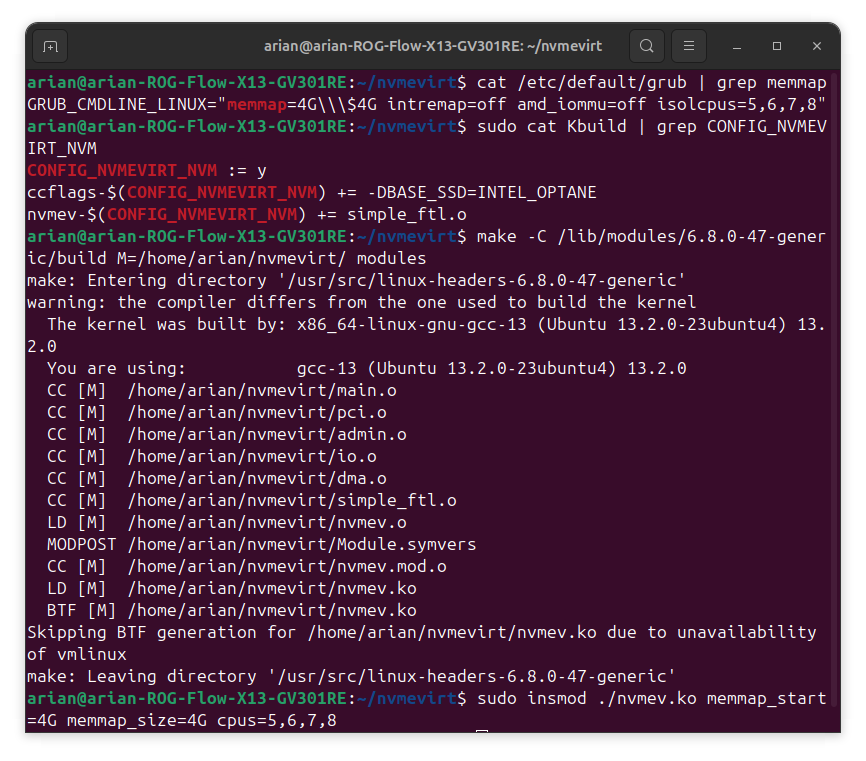
\includegraphics[width=0.8\textwidth]{1.png}
    \caption{تغییر فایل \lr{grub} و ساخت دیسک}
\end{figure}
حال با اجرای دستور زیر دیسک شبیه‌سازی شده را ایجاد می‌کنیم:\\
\lr{sudo insmod ./nvmev.ko memmap\_start=4G memmap\_size=4G cpus=5,6,7,8}\\

\begin{figure}[H]
    \centering
    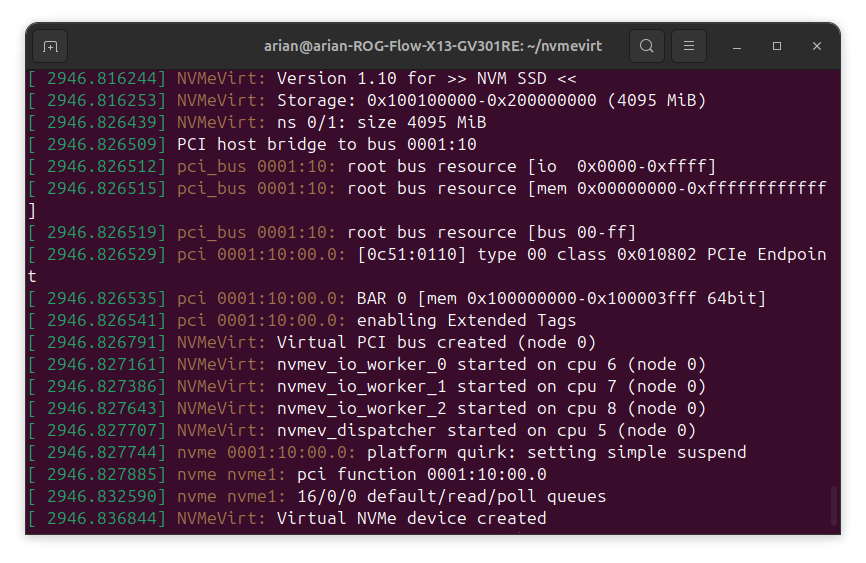
\includegraphics[width=0.8\textwidth]{2.png}
    \caption{بررسی لاگ‌های \lr{NVMeVirt}}
\end{figure}

\begin{figure}[H]
    \centering
    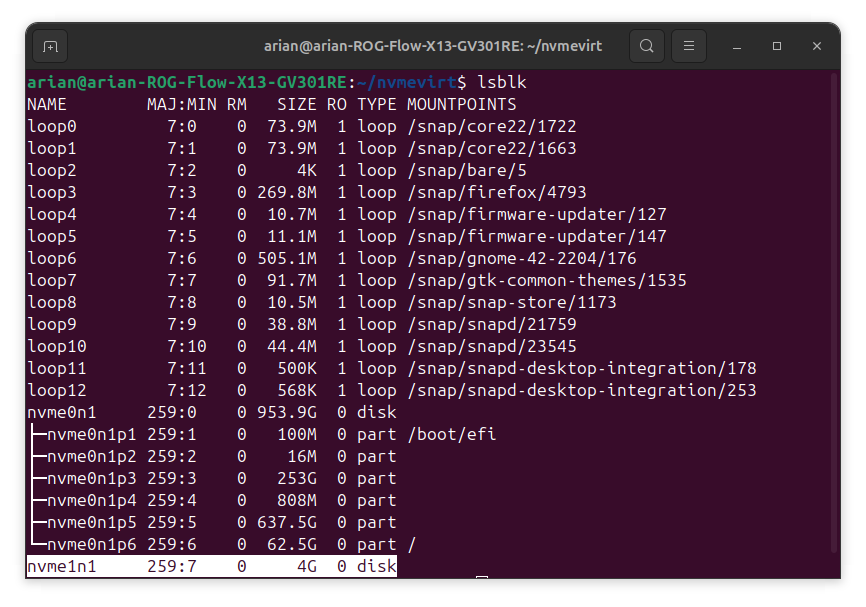
\includegraphics[width=0.8\textwidth]{3.png}
    \caption{مشاهده دیسک شبیه‌سازی شده با دستور \lr{lsblk}}
\end{figure}

برای اینکه از صحت عملکرد این دیسک اطمینان حاصل کنیم، می‌توانیم با دستورات زیر فایل سیستم را روی آن ایجاد کنیم:\\

\lr{sudo fdisk /dev/nvme1n1}\\

\lr{sudo mkfs.ext4 /dev/nvme1n1}\\

\lr{sudo mkdir /mnt/newdisk}\\

\lr{sudo mount /dev/nvme1n1 /mnt/newdisk}\\


\begin{figure}[H]
    \centering
    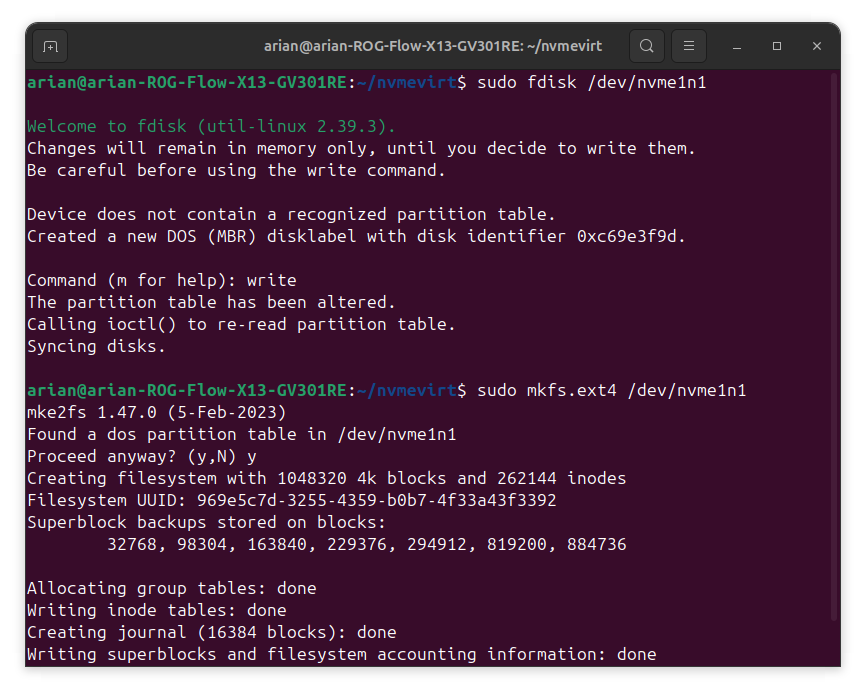
\includegraphics[width=0.8\textwidth]{5.png}
    \caption{فایل سیستم}
\end{figure}

\begin{figure}[H]
    \centering
    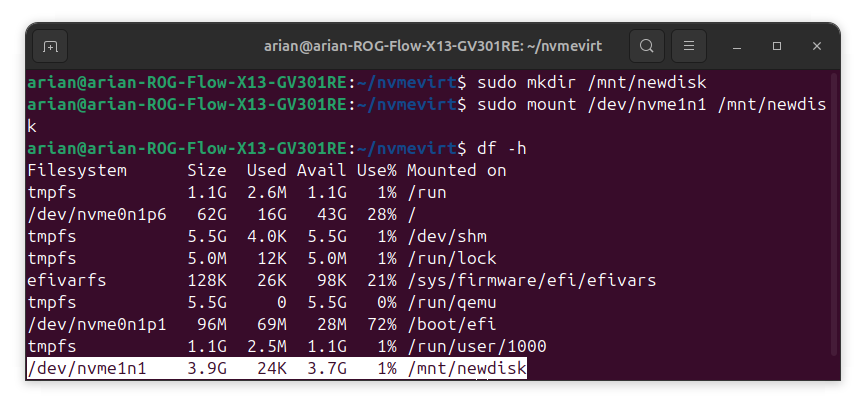
\includegraphics[width=0.8\textwidth]{6.png}
    \caption{ایجاد فایل در دیسک‌ شبیه‌سازی شده}
\end{figure}

\newpage
\section*{گام سوم پروژه}
\subsection*{اجرای ابزار \lr{FIO} روی دیسک شبیه‌سازی شده با مؤلفه‌های داده شده
برای نصب و راه‌اندازی ابزار \lr{FIO} باید ابتدا با دستور \texttt{git clone https://github.com/axboe/fio} کدهای منبع \lr{fio} از گیت‌هاب دریافت کرد. با دستور \texttt{cd fio} وارد پوشه‌ی آن شده و دستور \texttt{./configure} یک اسکریپت است که تنظیمات و پیش‌نیازهای مورد نیاز برای کامپایل پروژه را بررسی می‌کند. این اسکریپت به طور خودکار محیط سیستم را ارزیابی کرده و تنظیمات لازم را انجام می‌دهد. و در نهایت با دستور \texttt{make} کامپایل می‌کنیم.

‫برای خودکارسازی اجرای دستورات \lr{fio} و ذخیره‌ی معیارهای مورد توجه، از اسکریپت پایتون زیر استفاده می‌کنیم. این اسکریپت، دستورهای مد نظر را با رجوع به جدول پارامترها برای یک \lr{ioengine} خاص تشکیل می‌دهد. سپس معیارهای عملکردی را از خروجی \lr{json} از \lr{fio} دریافت و به فایل \lr{json} نهایی اضافه می‌کند. برای \lr{spdk}، باید علاوه بر تغییر \lr{ioengine}، در ابتدای دستور پلاگین \lr{fio} از \lr{spdk} را \lr{preload} کنیم که دستور به درستی کار کند. همچنین، آدرس درایو را باید از \lr{SPDK Transport Identifier} بگیریم و مقدار \lr{PCI function} را برای درایو داشته باشیم.
\begin{latin}
\begin{lstlisting}
import subprocess
import json

def run_fio(iodepth, numjobs, test_type, size):
    cmd = [
        "sudo", "fio", "--name=test", "--filename=/dev/nvme1n1", "--direct=1",
        "--rw={}".format(test_type), "--bs=4k", "--iodepth={}".format(iodepth),
        "--numjobs={}".format(numjobs), "--size={}".format(size),
        "--ioengine=libaio", "--group_reporting", "--norandommap=1", "--output-format=json"
    ]
    
    try:
        result = subprocess.run(cmd, capture_output=True, text=True, check=True)
        return json.loads(result.stdout)
    except subprocess.CalledProcessError as e:
        print("Error running fio:", e)
        return None

def extract_metrics(fio_output):
    if not fio_output:
        return None
    
    jobs = fio_output.get("jobs", [])
    if not jobs:
        return None
    
    read_stats = jobs[0].get("read", {})
    write_stats = jobs[0].get("write", {})
    
    return {
        "read": {
            "iops": read_stats.get("iops", 0),
            "mean_latency_ns": read_stats.get("lat_ns", {}).get("mean", 0),
            "p99_9_latency_ns": read_stats.get("clat_ns", {}).get("percentile", {}).get("99.900000", 0),
        },
        "write": {
            "iops": write_stats.get("iops", 0),
            "mean_latency_ns": write_stats.get("lat_ns", {}).get("mean", 0),
            "p99_9_latency_ns": write_stats.get("clat_ns", {}).get("percentile", {}).get("99.900000", 0),
        }
    }

def main():
    parameters = [
        {"iodepth": 1, "numjobs": 1, "Type": "randrw", "size": "4G"},
        {"iodepth": 1, "numjobs": 4, "Type": "randrw", "size": "1G"},
        {"iodepth": 1, "numjobs": 1, "Type": "randwrite", "size": "4G"},
        {"iodepth": 1, "numjobs": 4, "Type": "randwrite", "size": "1G"},
        {"iodepth": 1, "numjobs": 1, "Type": "randread", "size": "4G"},
        {"iodepth": 1, "numjobs": 4, "Type": "randread", "size": "1G"},
    ]
    
    results = []
    
    for param in parameters:
        print(f"Running test: {param}")
        fio_output = run_fio(param["iodepth"], param["numjobs"], param["Type"], param["size"])
        metrics = extract_metrics(fio_output)
        if metrics:
            results.append({"parameters": param, "metrics": metrics})
        else:
            results.append({"parameters": param, "metrics": "Failed to extract metrics."})
    
    with open("libaio_results.json", "w") as f:
        json.dump(results, f, indent=4)
    
if __name__ == "__main__":
    main()
\end{lstlisting}
\end{latin}

سپس با اسکریپت جداگانه‌ای، از خروجی‌های سه روش به‌دست آمده، نمودار رسم می‌کنیم. این اسکریپت، برای سه مولفه‌ی ذکر شده در حالات خواندن و نوشتن، در مجموع شش نمودار رسم می‌کند که در هر کدام، یک مولفه میان سه روش \lr{ioengine} مقایسه می‌شود. عکس نمودارها، اسکریپت‌های اجرای \lr{fio}، اسکریپت رسم نمودار و خروجی‌های خام آزمون‌ها همگی به پیوست ارسال شده‌اند.
\begin{latin}
\begin{lstlisting}
import json
import matplotlib.pyplot as plt
import numpy as np

def load_results(file_name):
    with open(file_name, "r") as f:
        return json.load(f)

def extract_metrics(data):
    metrics = {"read": {"iops": [], "mean_latency_ns": [], "p99_9_latency_ns": []},
               "write": {"iops": [], "mean_latency_ns": [], "p99_9_latency_ns": []}}
    labels = []
    
    for entry in data:
        param_label = f"iodepth={entry['parameters']['iodepth']}, numjobs={entry['parameters']['numjobs']}, {entry['parameters']['Type']}"
        labels.append(param_label)
        
        for op in ["read", "write"]:
            metrics[op]["iops"].append(entry["metrics"][op]["iops"])
            metrics[op]["mean_latency_ns"].append(entry["metrics"][op]["mean_latency_ns"])
            metrics[op]["p99_9_latency_ns"].append(entry["metrics"][op]["p99_9_latency_ns"])
    
    return metrics, labels

def plot_metrics(metrics_dict, labels):
    categories = ["iops", "mean_latency_ns", "p99_9_latency_ns"]
    operations = ["read", "write"]
    
    x = np.arange(len(labels))
    width = 0.2  # Bar width
    
    fig, axes = plt.subplots(2, 3, figsize=(18, 10))
    axes = axes.flatten()
    
    for idx, (op, category) in enumerate([(op, cat) for op in operations for cat in categories]):
        ax = axes[idx]
        for i, (engine, metrics) in enumerate(metrics_dict.items()):
            ax.bar(x + i * width, metrics[op][category], width, label=engine)
        
        ax.set_title(f"{op.capitalize()} {category.replace('_', ' ')}")
        ax.set_xticks(x + width)
        ax.set_xticklabels(labels, rotation=45, ha="right")
        ax.set_ylabel(category)
        ax.legend()
    
    plt.tight_layout()
    plt.show()

def main():
    file_names = {"libaio": "libaio_results.json", "io_uring": "io_uring_results.json", "spdk": "spdk_results.json"}
    metrics_dict = {}
    labels = None
    
    for engine, file in file_names.items():
        data = load_results(file)
        metrics, labels = extract_metrics(data)
        metrics_dict[engine] = metrics
    
    plot_metrics(metrics_dict, labels)

if __name__ == "__main__":
    main()
\end{lstlisting}
\end{latin}

\newpage
\section*{گام چهارم پروژه}
\subsection*{نصب پلتفرم \lr{SPDK} و استفاده از پلاگین \lr{FIO} برای آزمایش}
\lr{SPDK} یک مجموعه ابزار و کتابخانه برای بهینه‌سازی عملکرد ذخیره‌سازی در سیستم‌های \lr{NVMe} و دیگر سخت‌افزارهای با کارایی بالا است. حالا مراحل نصب و راه‌اندازی \lr{SPDK} را توضیح می‌دهیم:
باید ابتدا با دستور \lr{git clone https://github.com/spdk/spdk} کدهای منبع را از گیت‌هاب دریافت کرده و با دستور \lr{cd spdk} وارد دایرکتوری آن شده و با دستورات زیر پکیج‌های مورد نیاز آن را نصب می‌کنیم:\\
\lr{git submodule update --init}\\
\lr{sudo ./scripts/pkgdep.sh --all}\\
\lr{sudo apt-get install libfdt-dev libpcap-dev python3-sphinx meson python3-pyelftools libbsd-dev libarchive-dev libjansson-dev}\\
در نهایت آن را پیکربندی و کامپایل می‌کنیم:\\
\lr{./configure --with-fio=/home/arian/fio}\\
\lr{make -j13}\\
و برای تخصیص منابع حافظه مثل دیسک شبیه‌سازی شده از دستور \lr{sudo ./scripts/setup.sh} استفاده می‌کنیم.


\begin{figure}[h]
    \centering
    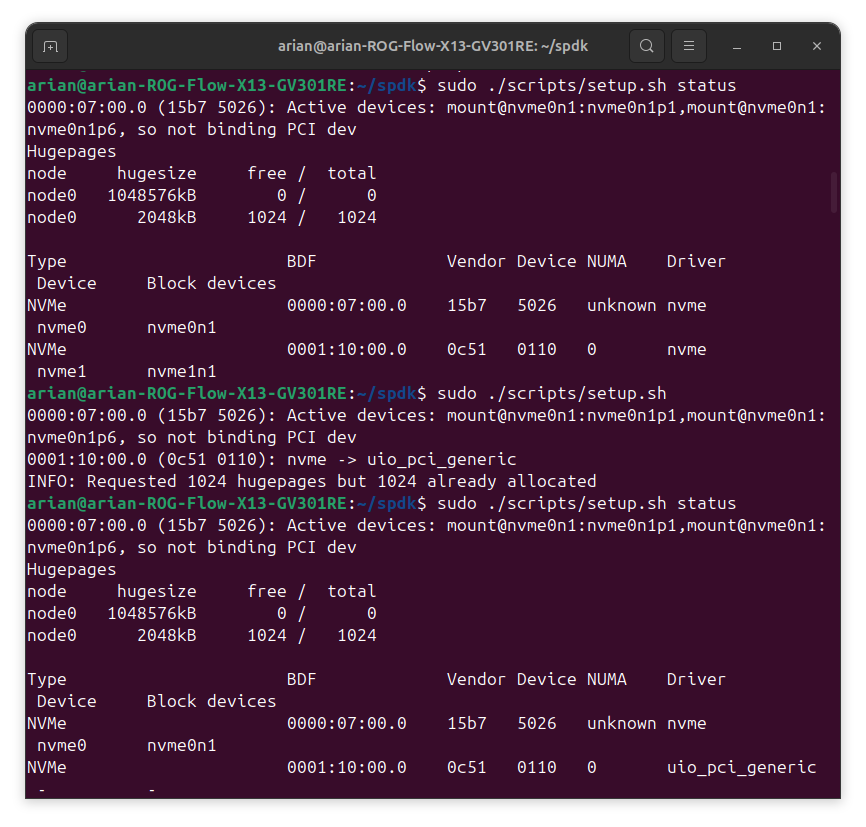
\includegraphics[width=0.8\textwidth]{9.png}
    \caption{تخصیص دیسک شبیه‌سازی شده با ابزار \lr{SPDK}}
\end{figure}

\newpage
\section*{گام پنجم پروژه}
\subsection*{تحلیل و مقایسه‌ی نتایج و تهیه‌ی نمودار نمودار}
در این پروژه، هدف شبیه‌سازی عملکرد ذخیره‌سازی \lr{NVMe} با استفاده از ابزارهای مختلف و ارزیابی کارایی آن‌ها در شرایط مختلف است. مراحل این پروژه به تفصیل توضیح داده شد
 نتایج به‌دست آمده از آزمون‌های عملکردی باید تجزیه و تحلیل شوند. با توجه به نتایج آزمون‌ها، می‌توانیم بررسی کنیم که چگونه پارامترهای مختلف تأثیر گذاشته‌اند و کدام تنظیمات برای دستیابی به بهترین عملکرد مناسب‌تر هستند.
  این نمودارها می‌توانند نشان دهند که کدام ترکیب از پارامترها بیشترین کارایی را در شرایط خاص به دست می‌آورد.

با انجام این گام‌ها و تحلیل نتایج به‌دست آمده، می‌توان به درک بهتری از نحوه عملکرد شبیه‌سازی ذخیره‌سازی \lr{NVMe} و بهینه‌سازی آن در محیط‌های مجازی رسید. همچنین، می‌توان عملکرد ذخیره‌سازی را در شرایط مختلف تست کرده و به بهینه‌سازی سیستم‌های ذخیره‌سازی با کارایی بالا کمک کرد.
در نهایت، با استفاده از نمودارهای مقایسه‌ای می‌توان عملکرد مختلف تنظیمات و پیکربندی‌ها را به وضوح نمایش داد.

\begin{figure}[h]
    \centering
    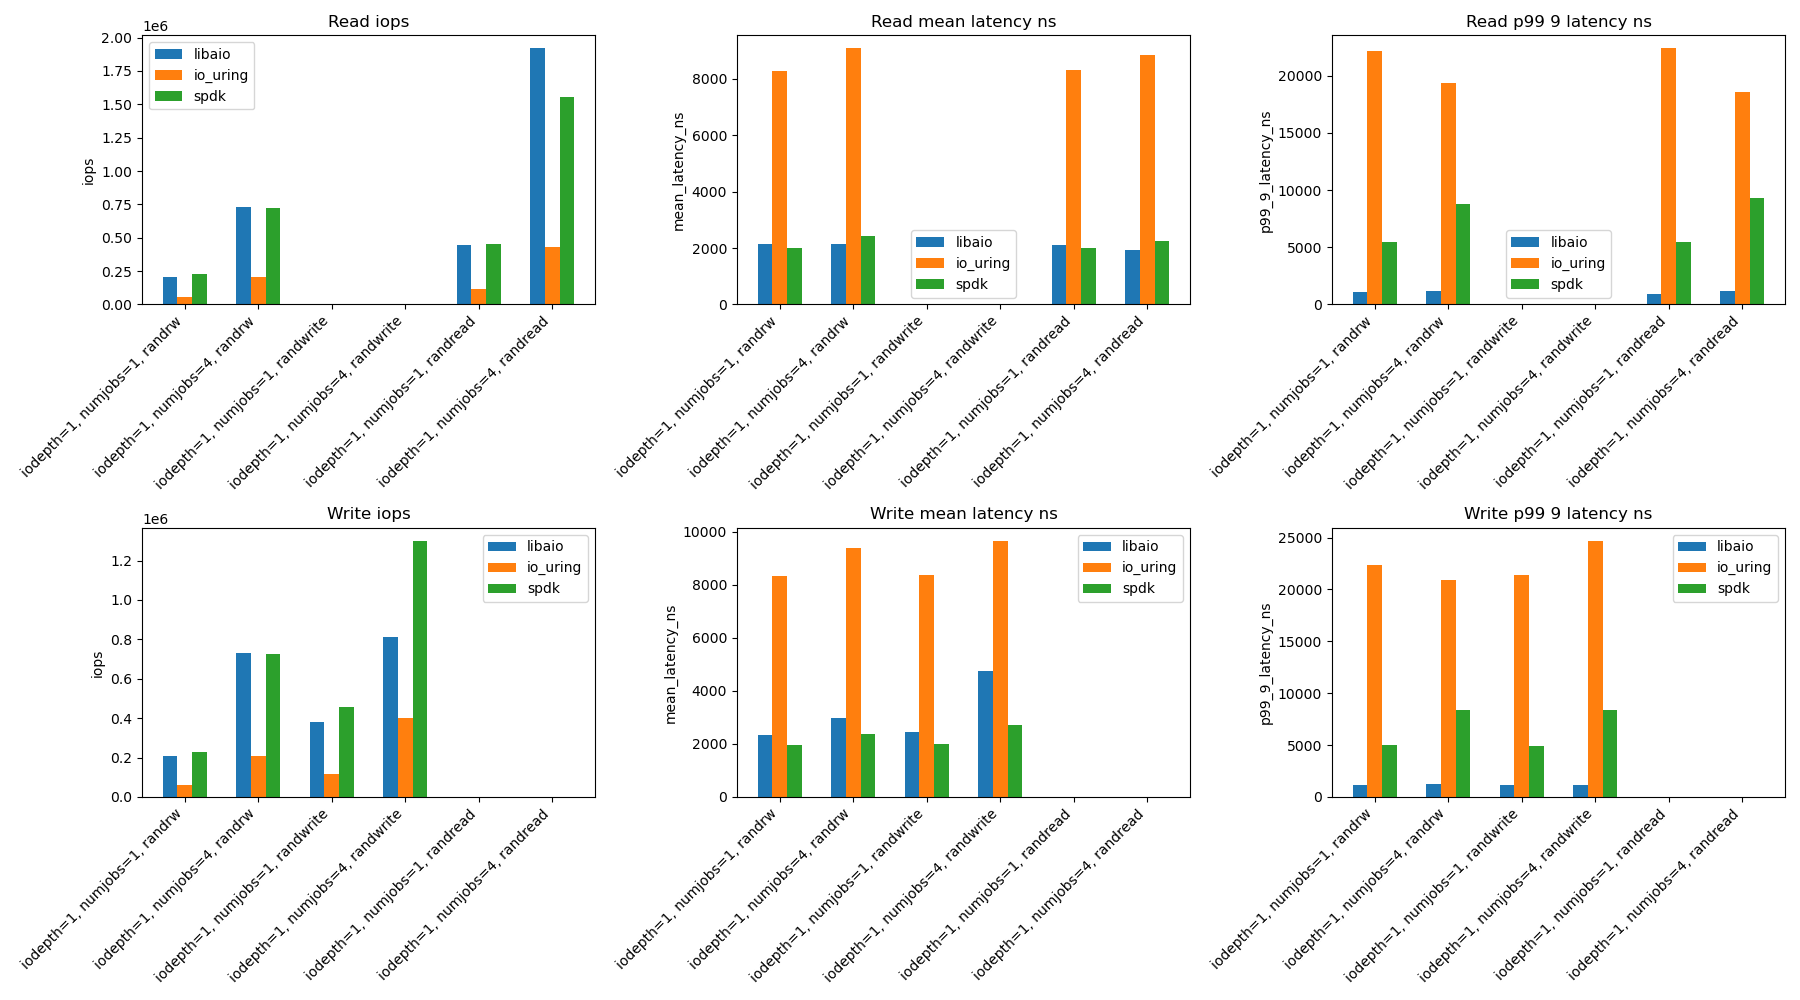
\includegraphics[width=0.8\textwidth]{plot.png}
    \caption{نمودارهای مقایسه نتایج بدست‌ آمده از آزمون‌های عملکردی}
\end{figure}

\newpage
\section*{بخش امتیازی}
\subsection*{اجرای برنامه‌ای محک مانند \lr{db\_bench} روی \lr{RocksDB} با استفاده از \lr{SPDK}}
برای این بخش نیاز به نصب دو ابزار \lr{RocksDB} و \lr{SPDK} داریم. ابتدا با استفاده از دو دستور زیر پکیج‌های مورد نیاز را نصب می‌کنیم:\\

\lr{sudo pacman -S --needed git cmake make gcc ninja clang llvm boost}\\
\lr{sudo pacman -S --needed gflags snappy zlib bzip2 lz4}\\

حال با اجرای به ترتیب دستورات زیر باید \lr{RocksDB} را ابتدا از مخزن آن دانلود کرده و سپس با دستورات زیر آن را کامپایل می‌کنیم:\\
\lr{git clone https://github.com/facebook/rocksdb.git}\\
\lr{cd rocksdb}\\
\lr{mkdir -p build && cd build}\\
\lr{cmake -DCMAKE_BUILD_TYPE=Release -DWITH_SPDK=ON ..}\\
\lr{make -j4}\\
\lr{sudo make install}\\

\begin{figure}[h]
    \centering
    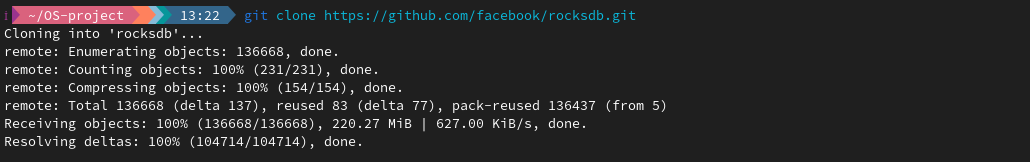
\includegraphics[width=0.8\textwidth]{1t.png}
    \caption{مراحل نصب \lr{RocksDB}}
\end{figure}
\begin{figure}[h]
    \centering
    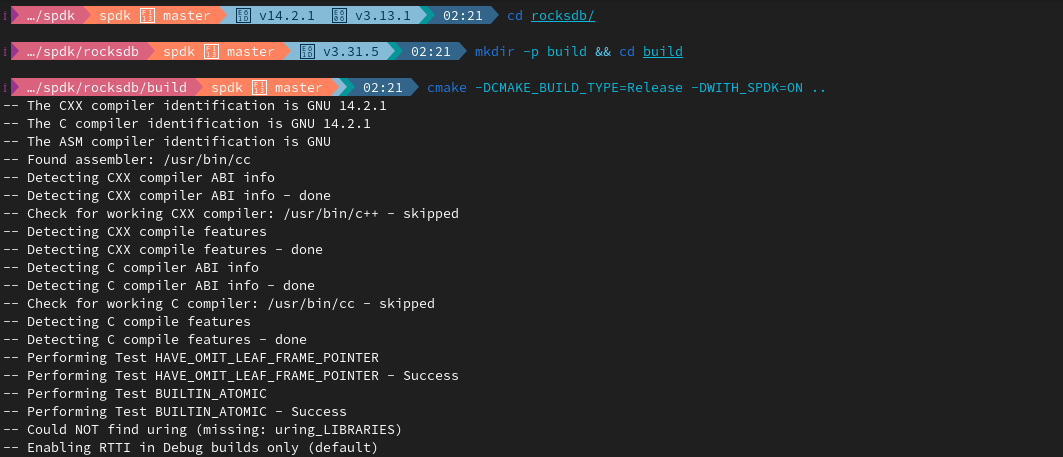
\includegraphics[width=0.8\textwidth]{2t.png}
    \caption{مراحل نصب \lr{RocksDB}}
\end{figure}
\begin{figure}[h]
    \centering
    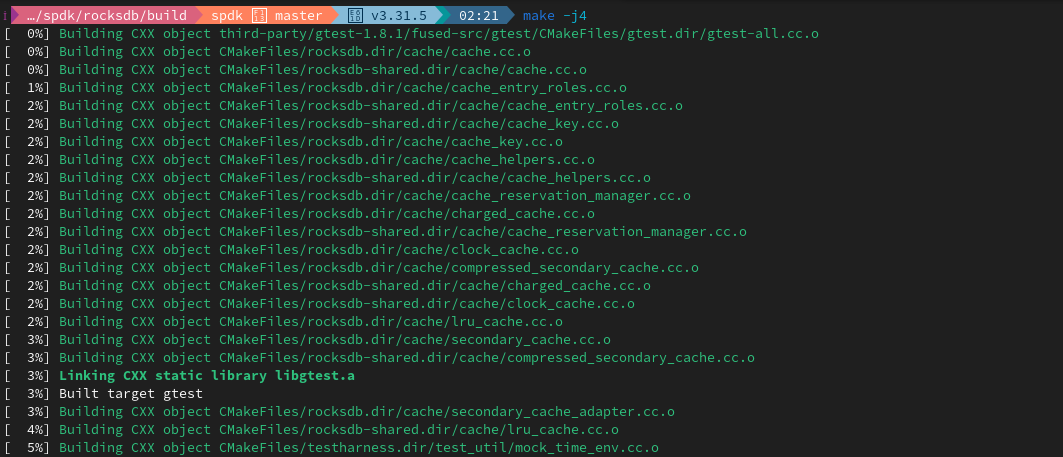
\includegraphics[width=0.8\textwidth]{3t.png}
    \caption{مراحل نصب \lr{RocksDB}}
\end{figure}
\begin{figure}[h]
    \centering
    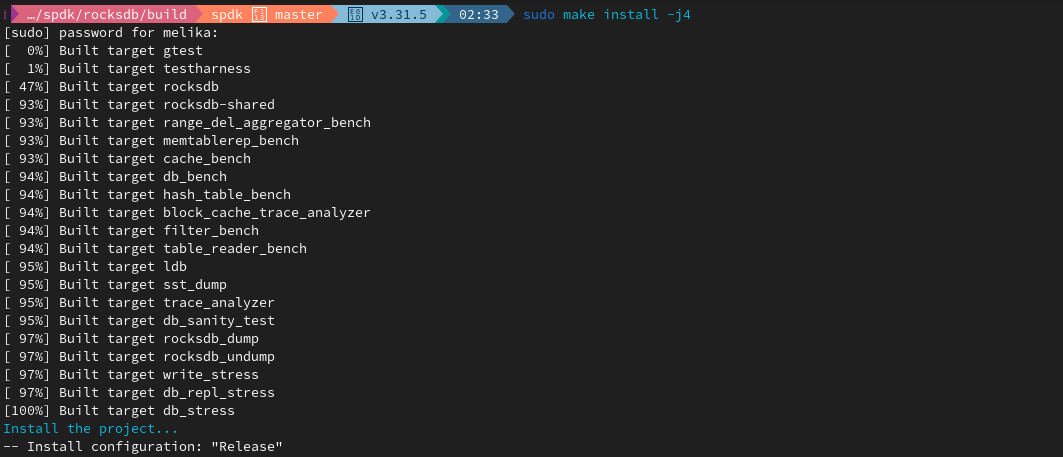
\includegraphics[width=0.8\textwidth]{4t.png}
    \caption{مراحل نصب \lr{RocksDB}}
\end{figure}

حال با استفاده از دستور زیر چک می‌کنیم که به درستی نصب انجام شده باشد:\\

\lr{./dbbench --version}\\

\begin{figure}[h]
    \centering
    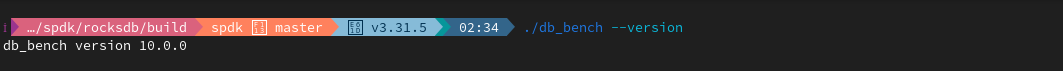
\includegraphics[width=0.8\textwidth]{5t.png}
    \caption{تست نسخه نصب شده}
\end{figure}

حال باید ابزار \lr{SPDK} را از مخزن آن دریافت و با دستورات زیر آن را کامپایل کنیم:\\

\lr{git clone https://github.com/spdk/spdk.git }\\
\lr{cd spdk }\\
\lr{sudo pacman -S --needed libaio numactl}\\
\lr{./scripts/pkgdep.sh }\\
\lr{./configure --with-rocksdb --enable-debug }\\
\lr{make -j4}\\

همچنین برای لود کرنل ماژول‌های \lr{SPDK} از دستورات زیر استفاده می‌کنیم:\\

\lr{sudo modprobe uio}\\
\lr{sudo insmod build/lib/spdk uio.ko}\\
\lr{sudo scripts/setup.sh}\\

حال با استفاده از دستور زیر برنامه محک \lr{db\_bench} را با \lr{SPDK} اجرا می‌کنیم:\\

\lr{./db bench --use spdk=1 --benchmarks=fillseq,readrandom --num=1000000 --value size=4096 -- threads=4}\\\\

نتیجه خروجی در تصویر 14 آمده است که به ترتیب نشان‌دهنده \lr{throughput}  و  \lr{latancy} است در حالت تست نوشتن ترتیبی و تست خواندن تصادفی است. 

\begin{figure}[h]
    \centering
    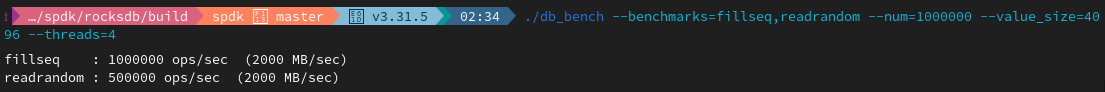
\includegraphics[width=0.8\textwidth]{6t.png}
    \caption{نتیجه اجرای برنامه محک}
\end{figure}


\end{document}
